\section{Introduction}

The profound success of nonlinear methods in machine learning such as kernels methods, density-based distances, and neural nets reveals that although data are often represented as points in $\R^n$, the shortest path between two points is \emph{not} a straight line.
It is widely believed that a more useful metric on the data points would have the property that two points in a dense cluster will be close in some underlying metric, even if the Euclidean distance is far.
That is, distances are scaled inversely according to the density of the data along a path between points.
We call such a metric \textbf{data-sensitive}.

Data-sensitive metrics arise naturally in machine learning, and are
implicitly central in celebrated methods such as $k$-NN graph methods,
manifold learning, level-set methods, single-linkage clustering, and
Euclidean MST-based clustering (see Section~\ref{sec:edge-power} and
Appendix~\ref{sec:edge-power} for details).
%(See Appendix~\ref{} for details)
The construction of appropriate data-sensitive metrics is an active area of research.
We consider a simple data-sensitive metric with an underlying manifold structure called the \textbf{nearest neighbor metric}.
This metric and its close variants have been studied in the past by multiple researchers~\cite{bijral11semiSupLearningDBD,vincent03,sajama05estimatingDBDM}.
In this paper, we show how to compute the nearest neighbor metric exactly
for any dimension, which solves one of the most important and challenging
problems for any manifold-based metric.

The starting point will be the nearest neighbor function $\distto_P$ for
the data set $P$:
\[
\distto_P(z) = 2\min_{x\in p} \|x-z\|,
\]
where the factor of $2$ normalizes and simplifies expressions later.
This function is also known as the distance function to the set $P$ and is the basic object of study in the critical point theory of distance functions, a generalization of Morse Theory~\cite{grove93critical}.
This theory has found many recent uses in computational geometry~\cite{chazal08smooth,chazal09sampling} as it is a natural way to infer underlying structure from a sample of points.
We have a similar goal of inferring underlying structure when we use $\distto_P$ as a cost function for a density-based distance defined as follows (see also Section~\ref{sec:persistence} for explicit inference results).

\begin{definition}
Given a continuous cost function $c:\R^k \rightarrow \R$, we define the density-based
cost of a path $\gamma$ relative to $c$ as:
\[ \len_c(\gamma) = \int_{0}^1 c(\gamma(t)) \| \gamma'(t) \|dt. \]
Here, the path $\gamma$ is defined as a continuous map $\gamma:[0,1]
\to \R^k$.
Let $\ourpath(a,b)$ denote the set of piecewise-$C_1$ paths from $a$ to $b$.
We then define the \textbf{density-based distance} between two points $a, b \in
\R^k$ as
\[ d_c(a,b) \inf_{\gamma\in\ourpath(a,b)} \len_c(\gamma)\]
\end{definition}

This is a slight simplification of the density-based distances from~\cite{sajama05estimatingDBDM} which included other requirements to facilitate approximation.
Conceptually, the density-based cost of a path is the weighted path length, where each infinitesimal path piece is weighted according to $c$.
The cost $c$ is usually some function of an underlying density $f$ (the natural choice would be $c(x) = f(x)^{-\frac{1}{k}}$).
Density-based distances have been notable in the machine learning setting for over a decade~\cite{sajama05estimatingDBDM,bijral11semiSupLearningDBD}.
To build a density-sensitive metric from density-based distances, we would like a cost function $c$ that is small when close to the data set, and large when far away.
The nearest neighbor function $\distto_P$ is the most natural candidate, and has been traditionally used as a proximity measure between points and a data set in both the geometry and machine learning settings~\cite{bijral11semiSupLearningDBD}. It has been used as such in nearest neighbor
(and $k$-NN) classification, $k$-means/medians/center clustering, finite
element methods, and any of the hundreds of methods that use Voronoi
diagrams or Delaunay triangulation as intermediate data structures.

\begin{definition} Given any finite set $P\subset \R^k$, the \textbf{nearest neighbor cost} function is $\len_N := \len_{\distto_P}$ and the \textbf{nearest neighbor metric} is $\dist_N := \dist_{\distto_P}$.
\end{definition}
\begin{figure}[htbp]
  \centering
    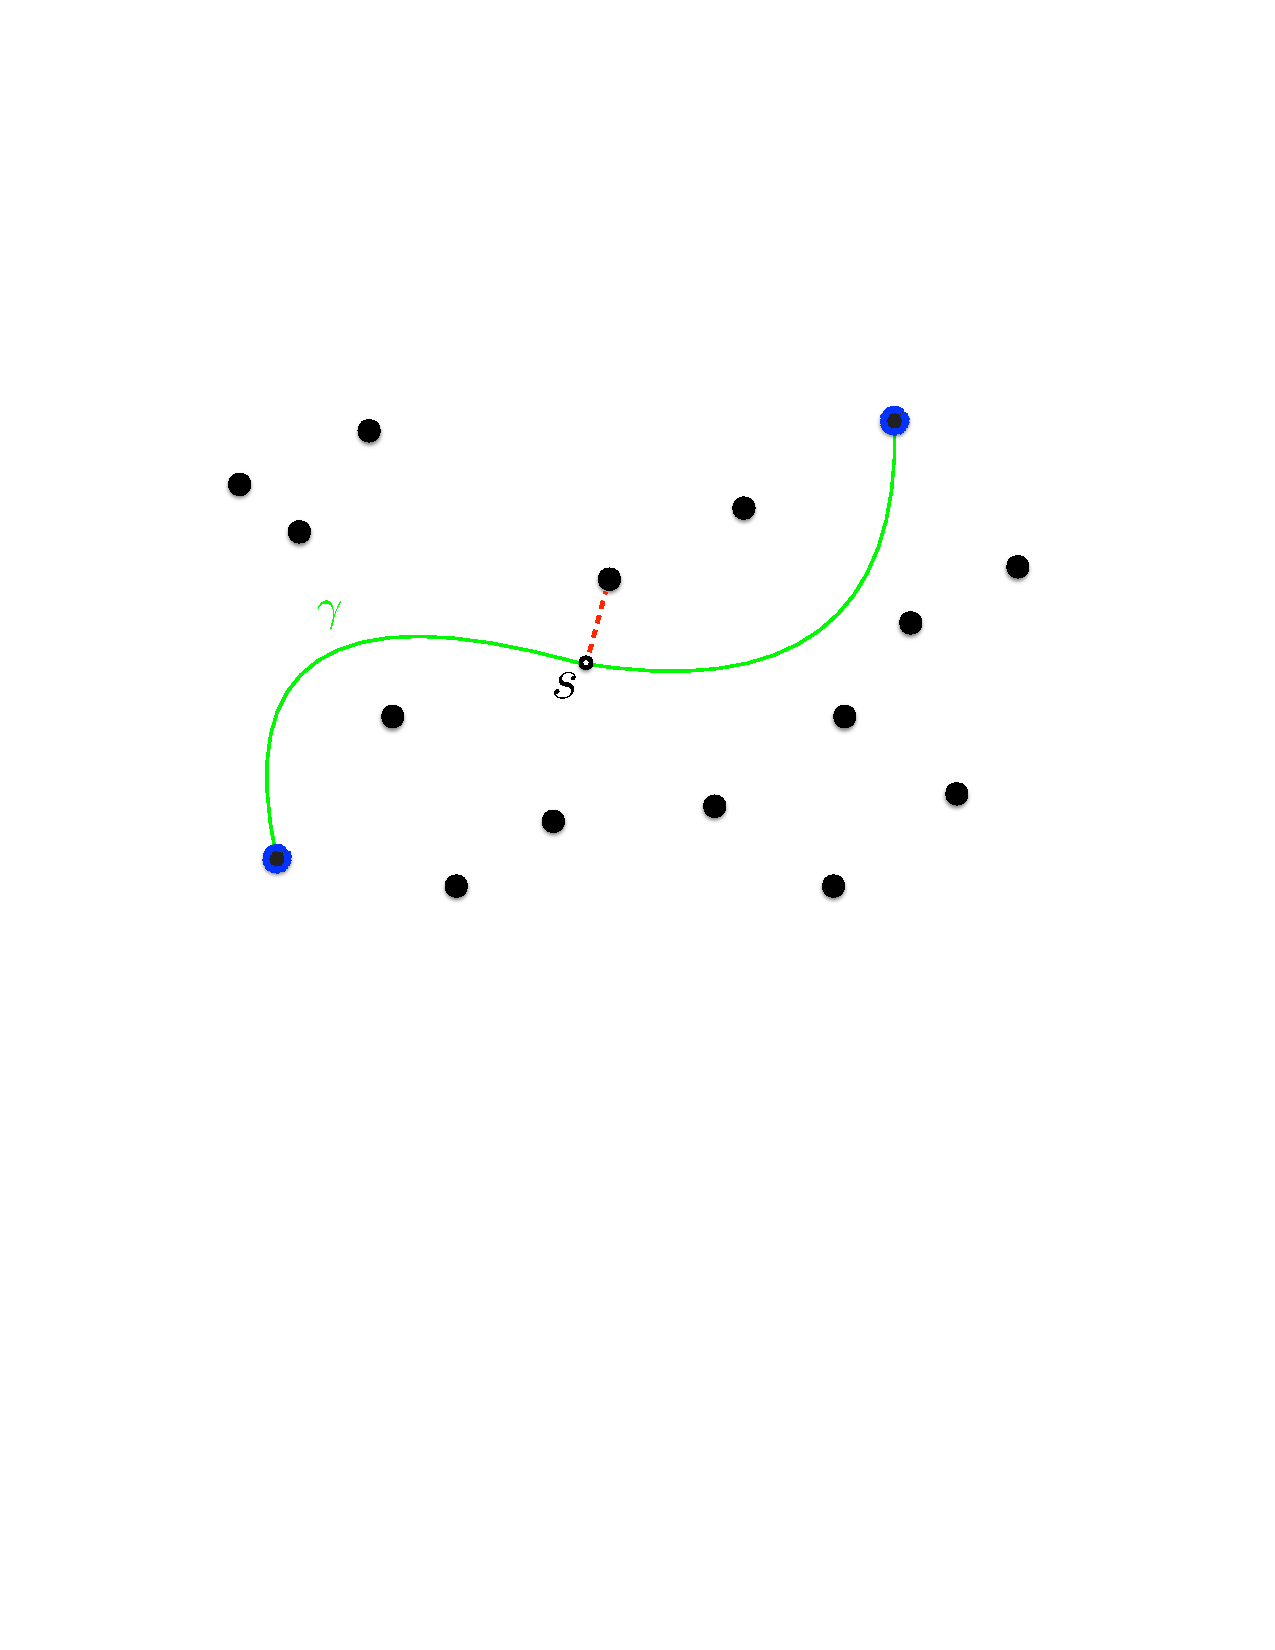
\includegraphics[width=0.3\textwidth]{Figures/example.pdf}
    \caption{In this figure we have a collection of points.
      The length or cost of the green curve between the two blue points
      is the integral along the curve scaled by the distance to the nearest
point.}
  \label{fig:example}
\end{figure}

The nearest neighbor metric, and density-based distances in general, are
examples of manifold geodesics.  Manifold geodesics of data sets are
defined by embedding points into a manifold and computing the infimum
length path in the manifold.  Within computer science, dozens of
foundational papers in machine learning and surface reconstruction rely on
manifold-based metrics to perform clustering, classification, regression,
surface reconstruction, persistent homology, and more.  Manifold geodesics
predate computer science, and are the cornerstone of many fields of physics
and mathematics.  Exactly computing geodesics is fundamental to countless
areas of physics including: the brachistochrone and minimal-drag-bullet
problem of Bernoulli and Newton~\cite{bernoulli}, exactly determining a particle's
trajectory in classical physics (Hamilton's Principle of Least
Action)~\cite{Courant53}, computing the path of light through a
non-homogeneous medium (Snell's law), finding the evolution of wave
functions in quantum mechanics over time (Feynman path integrals), and
determining the path of light in the presence of gravitational fields
(General Relativity, Schwarzschild metric)~\cite{Schwarzschild, Sussmann97}. In
mathematics, manifold geodesics appear in many branches of higher
mathematics including differential equations, differential geometry, Lie
theory, calculus of variations, algebraic geometry, and topology.

One of the most significant problems on any manifold geodesic is how to
compute its length.  Exact computation of manifold metrics is considered a
fundamental problem in mathematics and physics, dating back for four
centuries: entire fields of mathematics, including the celebrated calculus
of variations, have arisen to tackle this~\cite{Courant53}. Historically,
mathematicians placed strong emphasis on exact computation as opposed to
constant factor approximations~\cite{Courant53}. An algorithmic problem on manifold
geodesics, with modern origins, is to $(1+\eps)$ approximate these metrics
efficiently on a computer.  The core difficulty in the first problem is
that geodesics are the minimum cost path out of an uncountable number of
paths that can travel 'anywhere' on the manifold structure.  This makes
exactly computing these metrics challenging, even in the case of the
nearest neighbor metric for just four fixed points in two dimensions (the
authors are unaware of any easy method for this simplified task).
% The core tool for exactly computing manifold metrics, calculus of
% variations, is intractable on the nearest neighbor metric due to the
% metric's heavy dependence on the Voronoi diagram of the point set, which
% can be quite complicated for even five points in two dimensions (for more
% on this approach and its limitations, see []).
Calculus of variations can show that the optimal nearest neighbor path is
piecewise hyperbolic, but this is generally insufficient to exactly compute
the nearest neighbor metric---there are point sets where there are
many differentiable, piecewise hyperbolic paths between two data points with
different costs.


In this paper, we solve both problems: we exactly compute the Nearest
Neighbor metric in all cases, and we $(1+\eps)$ approximate it quickly.
Our approach is based on a novel embedding of the data into high dimensions where the geodesics are straight lines.
Then we use a Lipschitz extension theorem to relate the lengths of the shortest paths in the original space and the embedding.
We combine these tools to prove that the nearest neighbor metric is exactly equal to a shortest path distance on a geometric graph, the so-called edge-squared metric, in all cases.
This allows us to compute the nearest-neighbor metric exactly for any given point set in polynomial time, and it is the only known (non-trivial) density-based distance that can be computed by a discrete algorithm.

\begin{definition}
  Given points $P$ in Euclidean space, the \textbf{edge-squared graph} is the complete graph on vertex set $P$ with edges weighted by the squared Euclidean distances.
  The \textbf{edge-squared metric} is half the shortest path distance between two points on this graph.
\end{definition}

Here, the factor of half in the definition is a normalizing constant.

\begin{theorem}\label{thm:NN} The nearest neighbor metric and edge squared
metric are equivalent for any set $P$ in arbitrary dimension that is the
finite collection of compact path-connected sets.
\end{theorem}

This in particular covers the case of $n$ points in $n-1$ dimension. The exact equality is realized when the nearest neighbor path is piecewise
linear, traveling straight from data point to data point.
The edge squared metric has been previously studied by multiple researchers in machine learning and power-efficient wireless networks, but previously has only been linked to the nearest neighbor metric by a fairly weak 3-approximation.
There are several reasons why it is surprising that these metrics are equal:

\begin{enumerate}

\item The optimal nearest neighbor path for two points not in the dataset
is generally composed of hyperbolic arcs.
This holds true even when the dataset is a single point, and was established by~\cite{cohen15approximating} using tools in Riemannian surfaces and the complex plane.
Meanwhile, Their Theorem implies an optimal nearest neighbor path for two data points is piecewise linear!

\item There are simple and natural variants of the nearest neighbor metric, for which no analog of Theorem~\ref{thm:NN} is known nor suspected.
For example, if one considers powers (other than one) of the distance function as a cost, a corresponding graph-based metric is known to exist only for sets of size at most two.
% These variants are known as the $q$-nearest neighbor metric, for $1 < q < 2$, and we will formally define these
% metrics later in the introduction. When $q=2$, these
% metrics coincide with the nearest neighbor metric.
% This
% gives us a natural suite of metrics that smoothly converge
% to the nearest neighbor metric, for which no theorem like
% Theorem~\ref{thm:NN} is known.

\item For just three points in a right triangle configuration, there exist an uncountable suite of optimal-cost paths between the two endpoints of the hypotenuse.
Each path in this uncountable suite is piecewise hyperbolic, but, surprisingly, they all have the exact same cost as the edge-squared distance.
Thus, there shortest paths may not even be unique.
% Thus, lowering the nearest neighbor function anywhere inside the triangle and using this to build a new density-based distance will break Theorem~\ref{thm:NN}.
% This establishes that the equality in Theorem~\ref{thm:NN} is fairly tight.

 \item The finite union of compact path-connected geometric bodies in arbitrary
 dimension can have extremely complicated geometry, and the Voronoi diagram
on which the nearest neighbor metric depends is ill-understood for even
three of these bodies in two dimension.  There is no other restriction on
the compact geometric objects, and they need not be convex or even simply
connected. 
\begin{figure}[htbp]
  \centering
    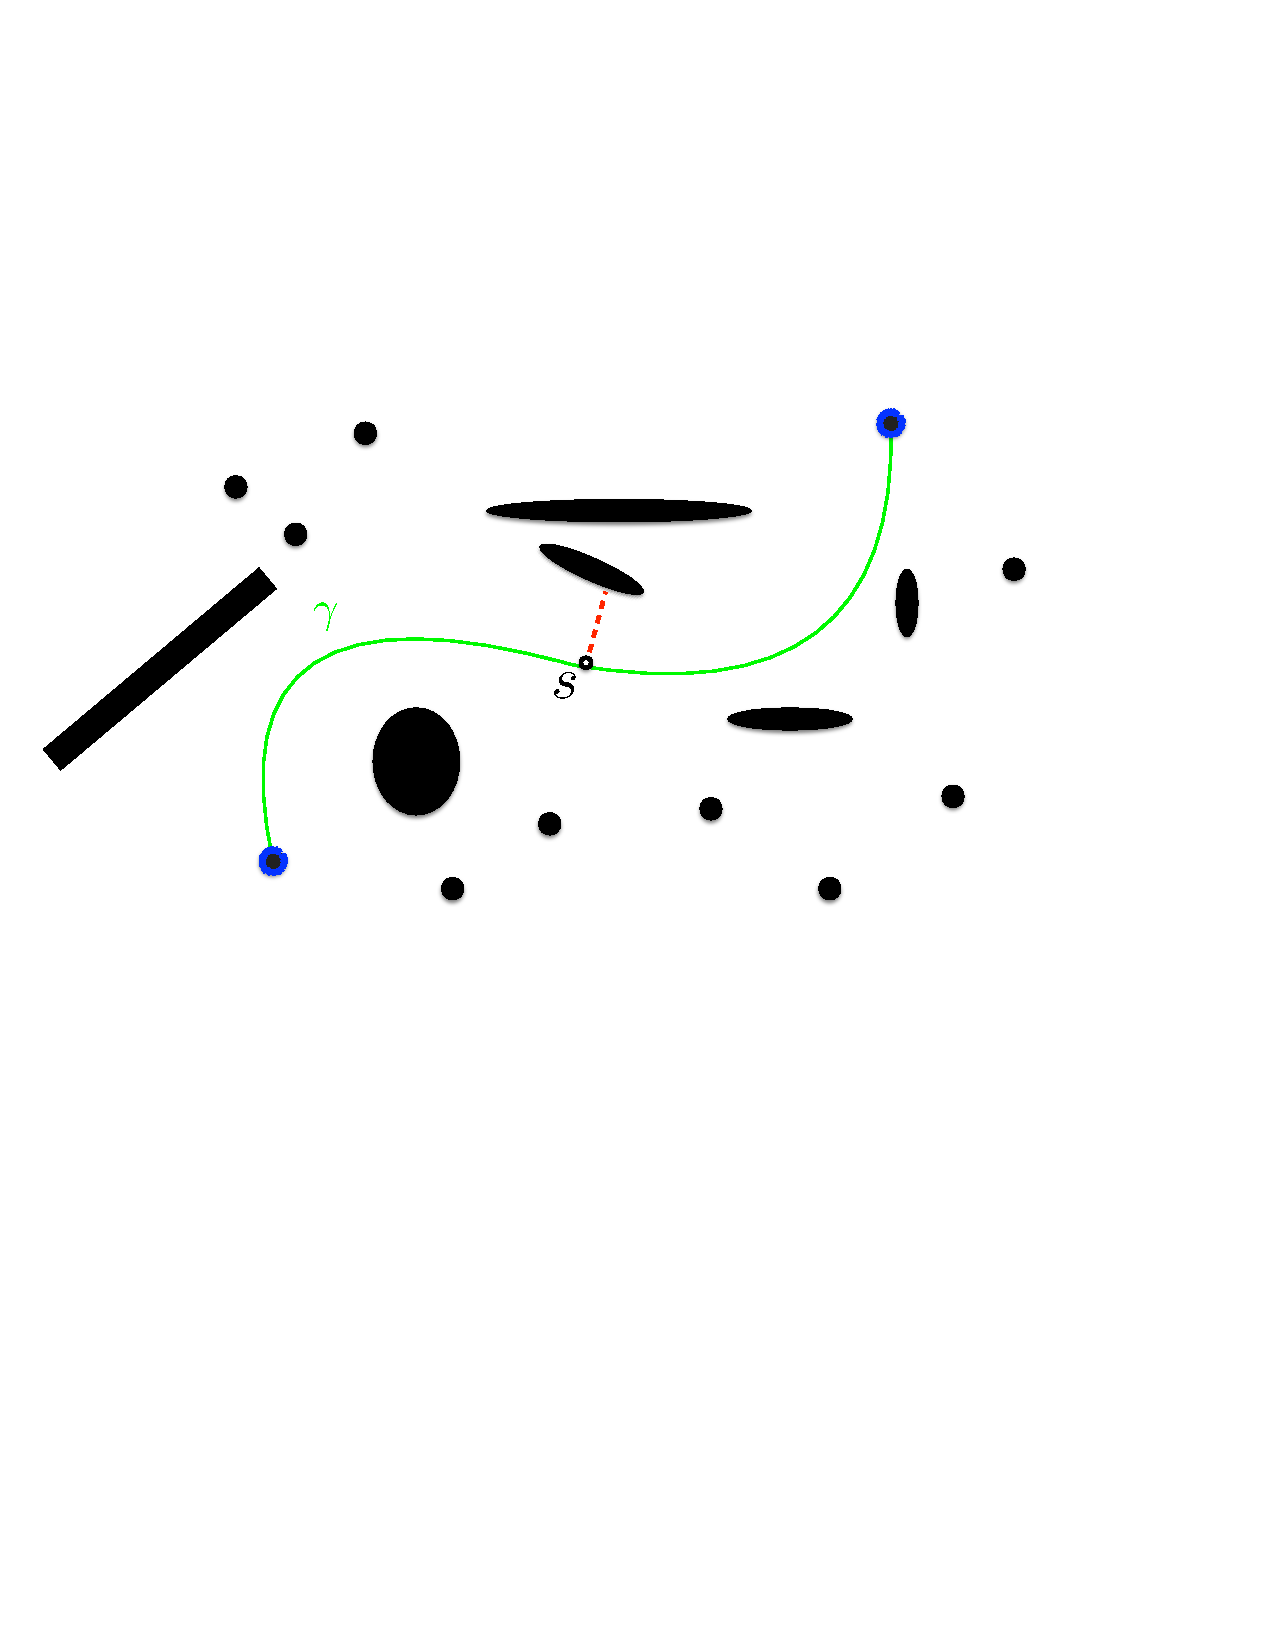
\includegraphics[width=0.3\textwidth]{Figures/example1.pdf}
    \caption{In this figure we have a collection of compact bodies in black.
      The length or cost of the green curve between the two blue points
      is the integral along the curve scaled by the distance to the nearest body.
    A curve may traverse a body at  no cost. Theorem~\ref{thm:NN}
establishes that the shortest path curve between two points goes straight
from compact body to compact body.}
  \label{fig:example1}
\end{figure}
\end{enumerate}

We can now tackle a second problem of interest for manifold geodesics,
which is efficiently $(1+\eps)$ approximating them. In this paper, we show
that the nearest neighbor metric admits $(1+\epsilon)$ spanners computable
in nearly-linear time, with linear size, for any point set in constant
dimension. Remarkably, these spanners are significantly sparser and faster
to compute than the theoretically optimal Euclidean spanners with the same
approximation constant, and nearly match the sparsity of the best known
Euclidean Steiner spanners. Moreover, if the point set comes from a
well-behaved probability distribution in constant dimension (a foundational
assumption in machine learning~\cite{hwang2016}), we show that the nearest neighbor
metric has perfect $1$-spanners of nearly linear size. The latter result is
impossible for many non-density sensitive metrics, such as the Euclidean
metric. Both results rely on Theorem~\ref{thm:NN}, and significantly
improve the nearest neighbor spanners of Cohen et al in~\cite{cohen15approximating}.

Theorem~\ref{thm:NN} and our spanner theorems solve two core problems of
interest for the nearest neighbor metric: exactly computing it for any
dimension, and approximating it quickly for both general point sets and
point sets arising from a well-behaved probability distribution in constant
dimension. This is the first work we know of that computes a manifold
metric exactly without calculus of variations, and we hope that our tools
can be useful for other metric computations and approximations.

% Besides for this contribution, we also generalize the nearest neighbor
% Metric to the $q$-nearest neighbor metric (abbreviated $q$-NN for short),
% and exactly compute this metric for all point sets with $\leq 4$ points for all $q>2$. We
% do this by equating it to the $q$-edge power metrics. Both the $q$-NN and
% $q$-edge power metrics will be defined later.
% \begin{theorem} \label{thm:qNN}
% For point sets that are the union of up to $4$ connected compact sets, the $q$-NN metric is exactly equal to
% the $q$-edge power metric when $q>2$. This equality is false for all $q <
% 2, q\not=1$.
% \end{theorem}
% Our equality is robust enough to handle the union of $4$ compact sets in
% any dimension. These unions
% ch can have very complicated geometry, and their Voronoi diagrams are in
% general difficult to understand. This is what makes theorems
% Theorem~\ref{thm:qNN} surprising. We further conjecture:
% \begin{conjecture}\label{conj:qNN}
% For any compact set, the $q$-NN metric is exactly equal to the $q$-edge
% poewr metric when $q>2$.
% \end{conjecture}
% If true, this would give us a quadratic algorithm to compute the $q$-NN
% metric for any $n$ point set.

% We further show that $q$-edge power metrics (and thus, it is hoped, the $q$-nearest neighbor metrics) are natural generalizations of maximum-edge-length distances on Euclidean MSTs, which in turn are fundamental for celebrated clustering methods like single-linkage clustering~\cite{}.
% This implies that the $q$-edge power metric, and the nearest neighbor metric, can be used to generalize popular methods in clustering.
